\section{Cieľ práce}
Všeobecným cieľom diplomovej práce je analyzovať existujúce riešenia virtuálnych laborato

Cieľom tejto práce je vytvorenie virtuálneho laboratória ako klient-server architektúru, kde server bude Node.js a klienti matlab a webová aplikácia v prehliadači. Experiment vrámci virtualného laboratória prebieha ako simulácia v Matlabe cez rozšírenie Simulink. Táto aplikácia nebude obmedzená len na lokálnu sieť, ale bude prístupna aj z internetu. Klient aj server bude vytvorený v dynamicky typovanom jazyku JavaScript. Údaje z experimentu sa budú zasielať z Matlabu na server cez websockety, kde môžu byť následne spracované a uložené do databázy, alebo zaslané klientovi do prehliadača.


\section{Virtuálne laboratória}
\indent V dobe keď internet ešte nebol rozšírený, experimenty sa robili vo fyzických laboratóriach. Bolo potrebné dodržiavať isté bezpečnostné predpisy, kvôli možnému úrazu osoby alebo možnému poškodeniu nástrojov.\\
\indent Vzdialenosť a hlavne nedostatok finančných zdrojov nám sťažuje podmienky pri testovaní experimentov, hlavne v prípadoch ked je potrebné mať pokrokové sofistikované nástroje. Ďalší problém s ktorým sa stretávame je nedostatok kvalitných lektorov. V dnešnej dobe existujú online kurzy, ktoré poskytujú aj video ukážky, ale to tento problém rieši len čiastočne. Vždy bolo výzvou vykonávanie spoločných experimentov viacerými inštitúciami súčasne a zároveň zdielanie nákladov na prostriedky. V súčasnej dobe internetu a počítačových technológií už tieto obmedzenia nemusia trápiť študentov ani výskumníkov. Internet umožnil to, že experimenty môžu byť štruktorované tak, aby boli ovládané a prezerané na ďiaľku. Práve to by pomohlo v učení v základných ale aj pokročilých konceptov prostredníctvom vzdialeného experimentovania. V súčasnosti veľa vybavenia už poskytuje rozhranie pre pripojenie počítača a spracovanie dát z neho. Vďaka tomu je možné navrhnúť experimenty, ktoré pomôžu študentom pri učení. Experimentovanie cez internet umožňuje využívanie zdrojov, znalostí, software a dát z  internetu narozdiel od fyzických experimentov, ktoré by vznikali súčasne na rôznych miestach.\cite{vlabphylosopfy}\\
\indent V tejto práci sa budeme zaoberať tvorbou virtuálneho laboratória (ďalej len VL). Predtým ako si popíšeme detailné fungovanie technológií pre vytvorenie VL, si musíme vysvetliť čo považujeme za VL, pochopiť aké hodnoty nám môže priniesť, ale samozrejme aj tie ktoré nemôže. Vo všeobecnosti môžme povedať ze VL je počítačový program, kde študenti sú v interakcii s experimentom prostredníctvom počítača. Typický príklad je simulácia experimentu, kedy je študent v interakcii s naprogramovaným rozhraním. Ďalšia možnosť je diaľkovo ovládaný experiment, kde študent je v interakcii s reálnym zariadením cez počítačové rozhranie, napriek tomu že sa nenachádza pri ňom. Keď vylúčime druhú variantu tak si môžme utvoriť definíciu nasledovne: \textit{Virtuálnym laboratóriom voláme to, keď je študent študent v interakcií s experimentom, ktorá je od neho fyzicky vzdialená alebo nemá za sebou žiadnu fyzickú realitu.}\cite{hatherly}

\begin{figure}[H]
  \centering
  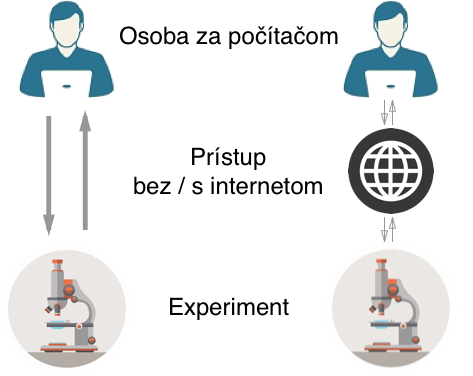
\includegraphics[scale=0.5]{img/VL_vs_real.png}
  \caption{Porovnanie medzi počítačovo riadneným experimentom vľavo a vzdialene riadeným experimentom vpravo.}
  \label{img-real-vs-vl}
\end{figure}

Po vysvetlení čo je VL sa pozrieme na výhody, ktoré nám môže priniesť. Sú popísané v bodoch v \textit{tabuľke č.\ref{table-real-remote-virtual-laboratory}.}
Človek často radí medzi "výhody" to, že môže nahradiť fyzické laboratória. Lenže to medzi výhody nepatrí. Nie je možné nahradiť skúsenosti z fyzickej práce zo zariadením VL aj keď je to lepšie ako žiadna skúsenosť. VL by nemalo byť vnímané tak, že poskytuje maximálnu možnú skúsenosť.
\begin{table}[H]
\small
\begin{tabular}{l l l}
\hline
\textbf{Typ laboratória} & \textbf{Výhody}  & \textbf{Nevýhody} \\ \hline
\textbf{Fyzické} & realistické dáta & obmedzenia na čase a mieste \\
& interakcia s reálnym zariadením & potrebné plánovanie prístupu\\
& lepšia spolupráca & nákladnosť experimentu \\
& interakcia s lektorom & potrebný lektor \\ \hline
\textbf{Virtuálne} & dobré pre vysvetlenie konceptu &  idealizované dáta\\
& bez obmedzenia na čas a miesto &  nedostatok spolupráce  \\
& interaktívne médium & bez interakcie s reálnym zariadením \\
& nízke náklady & \\ \hline
\textbf{Vzdialené} & interakcia s reálnym zariadením &  "virtuálna" prítomnosť v laboratóriu \\
& kalibrácia & \\
& realistické dáta & \\
& bez obmedzenia na čas a miesto & \\
& stredné náklady & \\ \hline
\end{tabular}
\caption{Porovnanie fyzických, virtuálnych a vzdialených a laboratórií}
\label{table-real-remote-virtual-laboratory}
\end{table}

\subsection{Prehľad existujúcich virtuálnych laboratórií}
V dobe písania tohto dokumentu existuje množstvo rôznych virtuálnych/vzdialených laboratórií, ktoré používajú zahraničné školy pre výučbu alebo výskum. V práci \cite{vlabtablecomparison} je zoznam veľmi používaných laboratórií, ktoré sú prístupne cez internet. Porovnanie funkcionality a využitých technológií je možné vidieť v  \textit{tabuľke č.\ref{table-vlab-comparison}.}

\begin{table}[H]
\scriptsize
\begin{tabular}{l l l l}
\hline\hline
\textbf{Názov} & \textbf{Klient} & \textbf{Server} & \textbf{Prevedenie}\\ \hline
Weblab-DEUSTO & AJAX, Flash, Java applets, & Web services, Python, LabVIEW, & Xilinx-VHDL, LabView\\
&LabVIEW, Remote panel & Java, .NET, C, C++ &\\ \hline
NCSLab & AJAX, Flash & PHP & Matlab, Simulink\\ \hline
ACT & HTML, Java Applets & PHP & Matlab, Simulink\\ \hline
LabShare Sahara & AJAX, Java applets & Web services, Java & Java\\ \hline
iLab & HTML, ActiveX, Java applets & Web services, .NET & LabVIEW\\ \hline
RECOLAB & HTML & PHP & Matlab, Simulink\\ \hline
SLD & AJAX, HTML & Web services, PHP & Matlab, Simulink\\ \hline\hline
\end{tabular}
\caption{Porovnanie virtuálnych laboratórií vytvorených mimo FEI STU.}
\label{table-vlab-comparison}
\end{table}

Následne som preskúmal možnosti existujúcich riešení v \textit{tabuľke č.\ref{table-feistu}}, ktoré boli vytvorené na Fakulte elektrotechniky a informatiky STU.\cite{table-vlab-farkas}\cite{table-vlab-borka}\cite{table-vlab-kundrat}\cite{table-vlab-cerveny}\cite{table-vlab-varga}
\begin{table}[H]
\tiny
\begin{tabular}{l l l l l l}
\hline\hline
\textbf{Rok vypracovania}  & \textbf{Autor} & \textbf{Prevedenie} & \textbf{Spôsob komunikácie} & \textbf{Klient} & \textbf{Server}\\ \hline
2011 &  Roman FARKAŠ & Matlab & JMI, sockets & Java & Java\\
&& Simulink &&& \\
&& Reálna sústava &&& \\ \hline
2012 &  Tibor BORKA  & Matlab & WCF & .NET, WPF & .NET\\
&& Simulink &&& \\
&& Reálna sústava &&& \\ \hline
2014 &  Michal KUNDRÁT  & Matlab & JMI, SOAP & HTML, JS & Tomcat, Java, \\
&& Simulink &&& JSF, EJB3\\ 
&&&&& MySQL\\ \hline
2014 &  Tomáš ČERVENÝ  & Matlab & JMI, HTTP & Mobilné HTML, JS & Jetty, Java\\
&& Simulink &&& \\ \hline
2015 &  Štefan VARGA  & Matlab & COM, HTTP & HTML, JS & PHP, .NET\\
&& Simulink &&& \\ \hline\hline
\end{tabular}
\caption{Porovnanie virtuálnych laboratórií vytvorených na FEI STU.}
\label{table-feistu}
\end{table}

\subsubsection{Nevýhody existujúcich riešení}
Pri tvorbe softwarového systému, či už všeobecne, alebo v našom prípade virtuálneho laboratória je vhodné preskúmať možnosti existujúcich riešení. Robí sa to kvôli tomu, aby sme sa pri návrhu vyvarovali rôznym chybám ktoré môžu nastať, alebo technológiam, ktoré už časom zastarali. V dnešnej dobe je vývoj nových technológií neskutočne rýchly. Takúto analýzu existujúch riešení sme spravili v predchádzajúcej sekcii.
Naša téma je zameraná na vytvorenie multiplatformového riešenia, kde nie je možné využiť WCF ani COM technológie ako v predchádzajúcich riešeniach. JMI je zase vhodné len pre riešenie, kde sa využíva Java. Pre server nie je možné využiť technológie LabVIEW, .NET (momentálne je vo vývoji multiplatformová verzia). Čo sa týka klienských riešení tak Flash, ActiveX, Java applets už nie sú podporované v prehliadačoch, taktiež ich nie je vhodné použiť.

\subsection{Komponenty virtuálneho laboratória}
Počet existujúcich laboratórií je veľký, ale väčšinou nie je možné zaručiť kompatibilitu, pretože tu neexistuje žiadny štandard. Ale vždy je možné identifikovať základné komponenty, ktoré tieto VL využívajú. Niektoré z nich môžu byť dokonca využité viac krát.\cite{article-components-vl}

\begin{enumerate}
  \item Samotný experiment
  \item Zariadenie umožnujúce kontrolu experimentu a získavanie hodnôt z neho.
  \item Laboratórny server, ktorý zabezpečí kontrolu, monitorovanie a spracovanie dát z experimentu.
  \item Server, ktorý zabezpečí prepojenie medzi vzdialenými uživateľmi a laboratórneho servera, zvyčajne prostredníctvom internetu.
  \item Webová kamera pripojená k serveru, ktorá môže byť použitá pre vzdialeného používateľa ako vizuálna a zvuková spätná väzba o stave experimentu.
  \item Nástroje umožňujúce viacužívateľské audio, video a chat komunikáciu.
  \item Klientské zariadenia, ktoré sa pripoja vzdialene k experimentu. Väčšinou sa jedná o webovú aplikáciu alebo java aplikáciu.
\end{enumerate}

Je ale dôležité si uvedomiť, že na vytvorenie laboratória nepotrebujeme všetky tieto komponenty, resp. môžme využiť aj iné, ktoré sa nám dokonale hodia. Niekedy sa používa napr. aj databázový server ak chceme experimenty ukladať a spracovávať neskôr. Tak isto je potrebné uvedomiť si, aký typ VL chceme vytvoriť. Určite budú rozdiely pri návrhu jednoužívateľského VL narozdiel od viacužívateľského dokonca s viacerými experimentami súčasne. Treba myslieť na to, ako vhodne vyriešiť škálovateľnosť, možné problémy s bezpečnosťou, viacužívateľský prístup, ostatné problémy prístupnosti a podobne.







\section{Použíté technológie}\label{used-technologies}

\subsection{Matlab R2015b}
\subsubsection{Simulink}
\subsubsection{Možnosti získania dát z workspace}

\subsection{Back-end}
\subsubsection{Node.js}
\subsubsection{MongoDB}

\subsection{Front-end}
\subsubsection{Angular.js}


\section{Návrh softwarového systému StarkLab}
\indent Témou práce je navrhnúť a implementovať virtuálne laboratórium s využiťím JavaScriptu na strane servera. V tejto kapitole si ukážeme predpokladaný návrh celého virtuálneho laboratória s využitím technológií na jednotlivých komponentoch. Ich presný popis a využitie si popíšeme viacej v \textit{sekcii č.\ref{used-technologies}}. Teda máme dané, že budeme využívať Node.js framework ako server. To je náš centrálny server (ďalej len StarkLab), ktorý spracováva dáta z Matlab workspace. Do Matlab workspace sú dáta posielané cyklicky zo Simulinku, v ktorom bola spustená referenčná schéma generujúca dáta. Nie je isté či bude možné docieliť spustenie Simulinku v reálnom čase multiplatformovo. Našli sme riešenie Simulink Real-time priamo od Mathworks, ktorá toto umožnuje ale bohužial len pre operačný systém Windows.\\
Na komunikáciu s workspace máme pri našom riešení dve možnosti. Buď volanie RESTful služieb, ktoré podporuje aj Matlab R2015b \cite{matlab-restful}, alebo websockets. Websockets by boli asi vhodnejšie pre túto komunikáciu kvôli rýchlosti, ale nie sú implementované priamo v matlabe, kvôli čomu musíme zanášať ďalšie knižnice do matlab path, ktoré sú implementované v Jave.\\
Komunikácia klienta a StarkLab môže bez problémov prebiehať cez websockets. Keď si užívateľ spustí simuláciu cez klienta, tak sa údaje budú uchovávať v databáze mongoDB pre neskoršie spracovanie.

\begin{figure}[H]
  \centering
  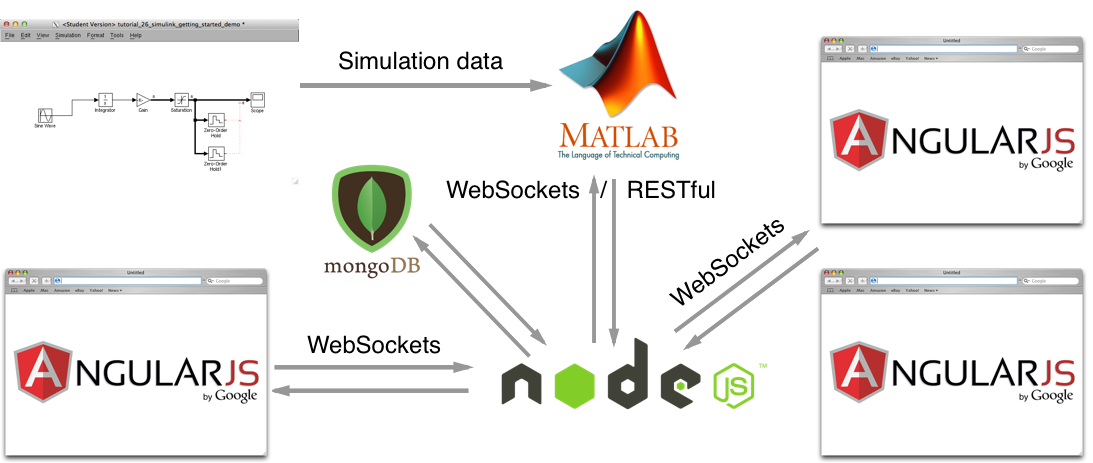
\includegraphics[scale=0.4]{img/software-design.png}
  \caption{Návrh komunikácie medzi jednotlivými komponentami.}
  \label{img-software-designl}
\end{figure}

\subsection{Diagramy}
\subsubsection{Use case}
\subsubsection{Activity}
\subsubsection{Model "class"}


\section{Implementácia}

\section{Testovanie}

\section{Inštalácia vytvoreného riešenia}